\section{Design Options}
\label{sec:options}

\subsection{Supersonic flow over a nose and wave drag}
\label{sec:physics}

Above $M = 1$, pressure disturbances can no longer travel upstream: a disturbance created at a point
only influences the region inside a downstream cone of half-angle
\begin{equation}
\mu = \arcsin\frac{1}{M},
\label{eq:mach}
\end{equation}
the \emph{Mach angle} ($\mu = 45.6^\circ$ at $M = 1.4$). The air ahead of the nose receives no
advance signal and is deflected abruptly through a \emph{shock wave}, across which pressure,
density and temperature jump. Where the surface turns back towards the axial direction, the flow
\emph{expands} and the pressure falls, possibly below ambient. The pressure on a supersonic nose is
therefore above ambient near the tip and decreases along it. Since the nose faces forward, this
gives a net axial force, the \emph{wave drag}, which exists even in an inviscid fluid. It is
expressed as $C_{D,\rm w} = D_{\rm w}/(q_\infty A_b)$ with the base area $A_b = \pi R^2$
(Equation~\eqref{eq:cdw}). Wave drag appears once the local flow becomes sonic somewhere on the
nose, around $M \approx 0.8$ for slender bodies, peaks near $M = 1$ and decreases slowly in the
supersonic range. It is the only drag component controlled by the nose shape.

A sharp, slender tip deflects the flow by a small angle and carries a weak oblique shock attached
to the tip. A blunt tip, or a half-angle too large for the Mach number, makes the shock detach into
a curved \emph{bow shock} whose central, normal part brings the flow almost to the stagnation
pressure. This is why supersonic noses are pointed and why any rounding of the tip has to stay
small (Section~\ref{sec:bluntness}).

For a slender nose, linearised (slender-body) theory makes the wave drag depend only on the axial
distribution of cross-sectional area $S(x) = \pi y(x)^2$, through $S''(x)$. Within a profile
family $S'' \propto R^2/L^2$, so
\begin{equation}
C_{D,\rm w} \propto \left(\frac{R}{L}\right)^2 \propto \frac{1}{(L/D)^2} :
\label{eq:fineness}
\end{equation}
doubling the length divides the wave drag by four. The area distribution of minimum wave drag is
also known: for a given length and base area it is the Von K\'arm\'an profile, with
$C_{D,\rm w} = 1/(L/D)^2$; for a given length and volume it is the LV-Haack profile. The theory
gives trends rather than exact values and is least accurate near $M = 1$; the Euler computations
of Section~\ref{sec:method} provide the values used in this study.

\subsection{Candidate profiles}
\label{sec:profiles}

The nose is defined by three choices: the \textbf{profile family}, the \textbf{fineness} $L/D$ and
the \textbf{tip bluntness} $r_n/R$. Seven profiles are compared (Table~\ref{tab:profiles},
Figure~\ref{fig:schematics}). With $\xi = x/L$ and $\eta = y/R$:
\begin{itemize}[leftmargin=*,itemsep=1pt]
\item \textbf{Conical}: straight generator of half-angle $\arctan(R/L)$ ($7.1^\circ$ at $L/D = 4$),
meeting the body with a kink of the same angle.
\item \textbf{Tangent ogive}: circular arc of radius $\rho = (R^2+L^2)/(2R)$, tangent to the body at
the shoulder; the traditional subsonic rocket nose.
\item \textbf{Parabolic series}: the case $K' = 1$ is the parabola tangent to the body at the shoulder.
\item \textbf{Power series} $\eta = \xi^n$: the smaller $n$, the fuller the front. For $n = \tfrac12$
the apex has a radius of curvature $R^2/(2L)$ (\SI{5.6}{mm} at $L/D = 4$), so this nose is blunt by
construction. Power noses meet the body with a kink $\theta_{\rm sh} = \arctan(nR/L)$.
\item \textbf{Haack series}: the minimum-wave-drag area distributions of slender-body theory, with
$C = 0$ (\textbf{Von K\'arm\'an}, given length and base area) and $C = \tfrac13$
(\textbf{LV-Haack}, given length and volume). Both are tangent at the shoulder; near the apex the
Von K\'arm\'an profile grows as $\xi^{3/4}$ (vertical tangent, zero tip radius).
\end{itemize}

\begin{figure}[tbp]
\centering
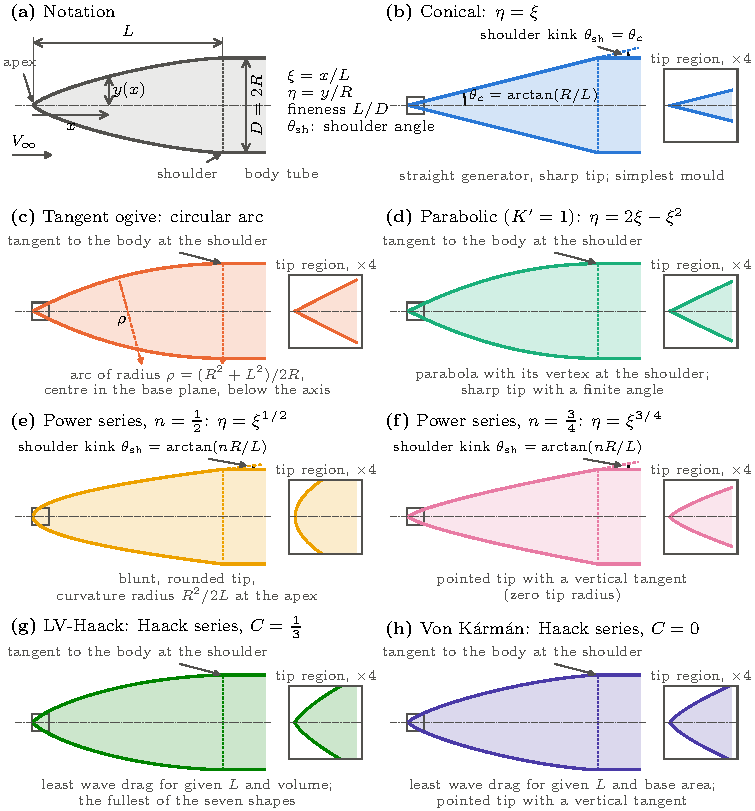
\includegraphics[width=\textwidth]{fig_schematics}
\caption{Schematics of the candidate profiles, drawn at $L/D = 2$ (half the design fineness) so
that their differences are visible; Figure~\ref{fig:gallery} shows them at real proportions.
(a) Notation. (b)--(h) Construction of each profile: the upper label describes the shoulder
(tangent to the body, or a kink of angle $\theta_{\rm sh}$), the lower label the generator and the
tip, and the inset shows the boxed tip region magnified four times.}
\label{fig:schematics}
\end{figure}

The profiles differ in three features (Figure~\ref{fig:schematics}): how the nose meets the body
(tangent, or with a kink), the shape of the tip (finite-angle point, pointed with a vertical
tangent, or blunt) and how the area is distributed along the length, from the thin cone to the
full LV-Haack nose. The elliptical nose (strong bow shock above Mach 1) and the secant ogive (no
advantage over the tangent ogive and LV-Haack, kinked shoulder) were discarded before computing.

\begin{table}[H]
\centering
\caption{Candidate profiles (ogive in dimensional form, $\rho$: arc radius). $x_{cp}$: Barrowman
nose centre of pressure; $\theta_{\rm sh}$: angle to the body at the shoulder (0 = tangent).}
\label{tab:profiles}
\small
\begin{adjustbox}{max width=\textwidth}
\begin{tabular}{@{}lllcc@{}}
\toprule
Profile & $\eta(\xi)$ & ERT vehicles & $x_{cp}/L$ & $\theta_{\rm sh}$ at $L/D=4$ \\
\midrule
Conical & $\xi$ & -- & 0.667 & $7.1^\circ$ \\
Tangent ogive & $\sqrt{\rho^2-(L-x)^2}+R-\rho$, $\rho=\frac{R^2+L^2}{2R}$ & Bella Lui II, Nordend & 0.464 & $0^\circ$ \\
Parabolic ($K'=1$) & $2\xi-\xi^2$ & -- & 0.467 & $0^\circ$ \\
Power series $n=\tfrac12$ & $\xi^{1/2}$ & Wildhorn, Firehorn & 0.500 & $3.6^\circ$ \\
Power series $n=\tfrac34$ & $\xi^{3/4}$ & -- & 0.600 & $5.4^\circ$ \\
LV-Haack ($C=\tfrac13$) & $\pi^{-1/2}\sqrt{\theta-\tfrac12\sin2\theta+C\sin^3\theta}$, $\theta=\arccos(1-2\xi)$ & -- & 0.438 & $0^\circ$ \\
Von K\'arm\'an ($C=0$) & as LV-Haack with $C=0$ & -- & 0.500 & $0^\circ$ \\
\bottomrule
\end{tabular}
\end{adjustbox}
\end{table}

\subsection{Comparison criteria}
\label{sec:criteria}

\begin{itemize}[leftmargin=*,itemsep=2pt]
\item \textbf{Wave drag.} At Weisshorn's Mach numbers it depends mostly on $L/D$ and on how much area
the profile adds near the tip. Slender-body theory makes Von K\'arm\'an the favourite; the Euler
computations check whether this holds at Weisshorn's finite thickness and Mach numbers.
\item \textbf{Volume and payload.} Fuller profiles reach $r=\SI{77}{mm}$ further forward, so more of
the 3U sits inside the curved part. The rest needs a cylindrical extension of the nose bay, which
adds vehicle length within the \SI{5.4}{m} cap.
\item \textbf{Stability.} Slender-body theory gives every nose that closes on $A_b$ the same
normal-force slope $C_{N\alpha} = 2$ per radian; the shape only sets where the force acts,
$x_{cp} = L - V/A_b$ from the apex ($2L/3$ for a cone). A fuller nose moves the vehicle CP forward
and lowers the static margin $(x_{cp} - x_{cg})/D$.
\item \textbf{Manufacture.} A tangent shoulder ($\theta_{\rm sh}=0$) avoids a kink at the coupler bond
line, a fillet in the mould and a local expansion in the flow. A sharp tip cannot be laid up in
prepreg, so every option uses a separate machined tip.
\end{itemize}
